%%%%%%%%%%%%%%%%%%%%%%%%%%%%%%%%%%%%%%%%%%%%%%%%%%%%%%%%%%%%%%%%%%%%%%%%%%%%%%%%%%%%%%%%%%%%%%%%
\section{Die elektrische Ladung}
Atome beinhalten Kerne aus Nukleonen, nämlich aus Protonen und Neutronen, und um den Kern herum aus Elektronen. \textbf{Protonen} haben positive Ladung, \textbf{Neutronen} haben neutrale Ladung und \textbf{Elektronen} haben eine negative Ladung. Die Summe aller den Kern umkreisenden Elektronen bezeichnet man als \textbf{Elektronenhülle}. Die Kernbindung bleibt stabil aufgrund der starke Wechselwirkung zwischen den Nukleonen.
% \begin{wrapfigure}{o}{7cm}
% 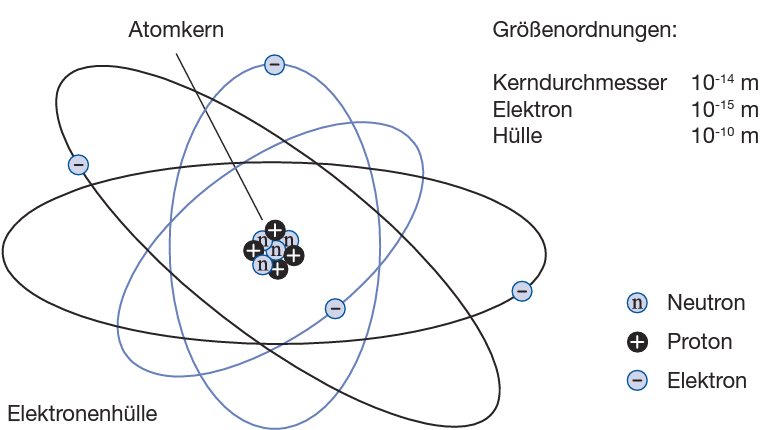
\includegraphics[scale=0.5]{../img/I/Ia}
% \centering
% \caption{Das Bohr'sche Atommodell}
% \label{fig_Ia}
% \end{wrapfigure}
\begin{figure}[H]
\centering
\frame{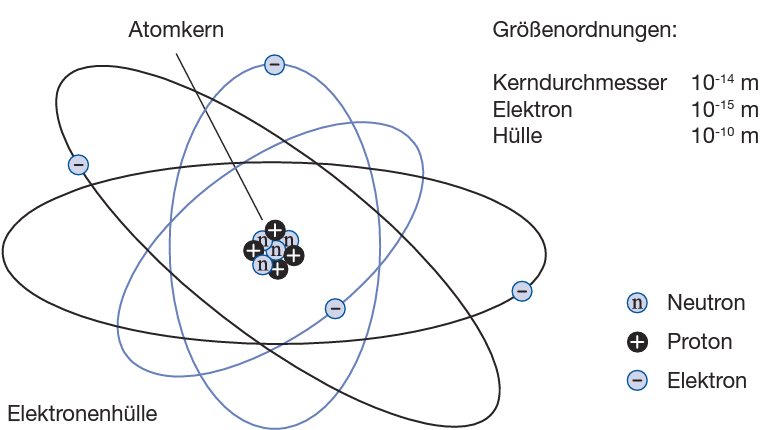
\includegraphics[scale=0.5]{../img/I/Ia}}
\caption{Das Bohr'sche Atommodell}
\label{fig_Ia}
\end{figure}
\noindent Die \textbf{Elementarladung} $e$ ist die kleinste Ladungsmenge. Die Atome verhalten sich neutral dank der positiven Ladung der Protonen $+e$ und der negativen Ladung der Elektronen $-e$. Die \textbf{Ordnungszahl} ist die Anzahl an Protonen oder an Elektronen. Der Wert der Elementarladung $e$ ist konstant und unabhängig vom Bewegungszustand des Teilchens. Die Teilchenmasse ist abhängig von der Geschwindigkeit bzw. der Bewegungszustand.
\begin{equation}
\boxed{e=1,60221892\cdot 10^{-19}\text{As}}
\end{equation}
Durch chemische Reaktionen werden die Elektronen von den Atomen getrennt. Bei einem \textbf{Elektronenüberschuss} entstehen Kräfte als bei einem \textbf{Elektronenmangel}. Ladungen gleichen Vorzeichens stossen sich gegenseitig ab. Ladungen unterschiedlichen Vorzeichens ziehen sich gegenseitig an.
%%%%%%%%%%%%%%%%%%%%%%%%%%%%%%%%%%%%%%%%%%%%%%%%%%%%%%%%%%%%%%%%%%%%%%%%%%%%%%%%%%%%%%%%%%%%%%%%
\section{Das Coulomb'sche Gesetz}
Die Kraft zwischen Ladungen $Q_1$ und $Q_2$ ist betragsmässig proportional zu jeder der beiden Ladungen und umgekehrt proportional zum Quadrat des Abstandes $r$ zwischen den Ladungen. Der Faktor $\epsilon_0$ ist die \textbf{elektrische Feldkonstante} oder Dielektrizitätskonstante des Vakuums.
\begin{equation}
\boxed{F=k\cdot \dfrac{Q_1Q_2}{r^2},\quad k=\dfrac{1}{4\pi\epsilon_0}}\quad \boxed{\epsilon_0=8,854\cdot 10^{-12}\text{AsV}^{-1}\text{m}^{-1}}
\end{equation}
\begin{figure}[H]
\frame{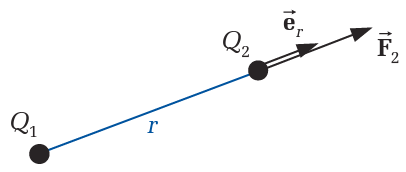
\includegraphics[scale=0.5]{../img/I/Ib}}
\centering
\caption{Zwei Punktladungen gleichen Vorzeichens}
\label{fig_Ib}
\end{figure}
\noindent Es wird angenommen, dass die geometrische Ausdehnung der Ladungen viel kleiner als der Abstand zwischen den Ladungen ist, daher spricht man von der Kraft zwischen \textbf{Punktladungen}. Mit der Festlegung eines Einheitsvektors {0}{7cm}$\overrightarrow{e}_r$ kann die Kraft von der Punktladung $Q_1$ auf die Punktladung $Q_2$ zeigen. Haben beide Ladungen gleiche Vorzeichen, so wird die Ladung $Q_2$ von der Ladung $Q_1$ abgestossen. \\Haben beide Ladungen unterschiedliche Vorzeichen, so wird die Ladung $Q_2$ von der Ladung $Q_1$ angezogen und die Kraft wirkt entgegengesetzte Richtung $-\overrightarrow{e}_r$ wirken.
\begin{equation}
\boxed{\overrightarrow{F}_2=k\cdot \dfrac{Q_1Q_2}{r^2}\cdot \overrightarrow{e}_r=\overrightarrow{E}_1\cdot Q_2}\quad \boxed{\overrightarrow{E}_1=k\cdot \dfrac{Q_1}{r^2}\overrightarrow{e}_r}
\end{equation}
%%%%%%%%%%%%%%%%%%%%%%%%%%%%%%%%%%%%%%%%%%%%%%%%%%%%%%%%%%%%%%%%%%%%%%%%%%%%%%%%%%%%%%%%%%%%%%%%
\section{Die elektrische Feldstärke}
Die zeitliche Abhängigkeit der Lage von Ladungen wird durch einen \textbf{elektrischen Feld} $\overrightarrow{E}$ beschrieben unabhängig von der Wahl des Koordinatensystems. Durch den Raum und Material wird zu jedem Zeitpunkt die Lage der Punktladungen bestimmt. Die \textbf{elektrische Feldstärke} $\overrightarrow{E}$ hat die Dimension $\text{Vm}^{-1}$. Das elektrostatische Feld existiert auch wenn bei der Abwesenheit von Punktladungen keine Kräfte entstehen.
\newline\newline
Eine positive Punktladungruft im homogenen Raum eine radial nach aussen gerichtete elektrische Feldstärke hervor, die mit dem Quadrat des Abstandes von der Punktladung abnimmt. Bei einer negativen Punktladung zeigt der Feldstärkevektor zur Punktladung hin.
\newline\newline
Die elektrische Feldstärke $\overrightarrow{E}$ beschreibt die \textbf{Wirkung} des elektrischen Feldes. Sie ist eine \textbf{Intensitätsgrösse} und wird gemessen durch die auf Ladungen ausgeübte Kraftwirkung. 
\newline\newline
Die Kraft auf eine positive Punktladung hat die gleiche Richtung wie die elektrische Feldstärke an der Stelle der Punktladung. Bei einer negativen Punktladung zeigen Feldstärke und Kraft in entgegengesetzte Richtungen.
%%%%%%%%%%%%%%%%%%%%%%%%%%%%%%%%%%%%%%%%%%%%%%%%%%%%%%%%%%%%%%%%%%%%%%%%%%%%%%%%%%%%%%%%%%%%%%%%
\section{Überlagerung von Feldern}
Befindet sich eine Punktladung $Q_1$ im Ursprung des Kugelkoordinatensystems, so ruft sie die Feldstärke hervor. Der Vektor $\overrightarrow{e}_r$ entspricht dem radialen Einheitsvektor des Kugelkoordinatensystems. Befindet sich die Punktladung $Q_1$ an der Quellenpunktskoordinate $\overrightarrow{r}_Q$ und der Aufpunkt $P$ mit Aufpunktskoordinate $\overrightarrow{r}_P$, an dem das Feld berechnet werden soll, dann ist die Richtung der Feldstärke im Aufpunkt $P$ durch den Einheitsvektor $\overrightarrow{e}_r$ und die Feldstärke $\overrightarrow{E}\left(\overrightarrow{r}_P\right)$
\begin{equation}
\boxed{\overrightarrow{e}_r=\dfrac{\overrightarrow{r}_P-\overrightarrow{r}_Q}{\Big\vert\overrightarrow{r}_P-\overrightarrow{r}_Q\Big\vert}=\dfrac{\overrightarrow{r}}{\Big\vert \overrightarrow{r}\Big\vert}=\dfrac{\overrightarrow{r}}{r}}
\end{equation}
\begin{equation}
\boxed{\overrightarrow{E}\left(\overrightarrow{r}_P\right)=\overrightarrow{e}_r\cdot k\cdot \dfrac{Q_1}{r^2}=\dfrac{\overrightarrow{r}}{r}\cdot k\cdot \dfrac{Q_1}{r^2}=k\cdot Q_1\cdot \dfrac{\overrightarrow{r}}{r^3}}
\end{equation}
\begin{figure}[H]
\frame{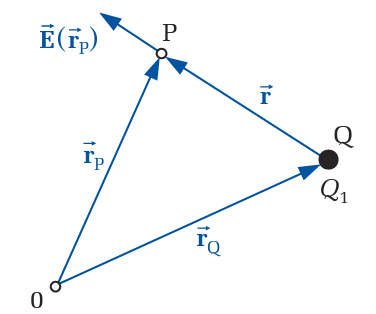
\includegraphics[scale=0.6]{../img/I/Ih}}\quad
\frame{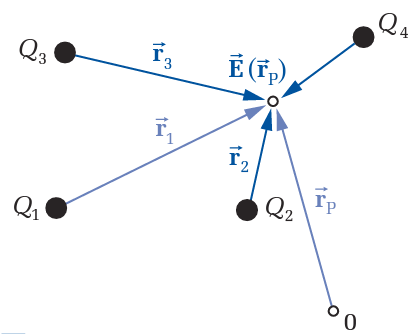
\includegraphics[scale=0.55]{../img/I/Ic}}
\centering
\caption{\textbf{\textit{Links:}} Berechnung der Feldstärke im Aufpunkt $P$. \textbf{\textit{Rechts:}} Kräfte mehrerer Punktladungen}
\label{fig_Ih}
\end{figure}
\noindent Sind $3$ Ladungen $Q_1$, $Q_2$ und $Q_3$ an den Stellen $\overrightarrow{r}_{Q_i}$ vorhanden, dann erhält man die Gesamtkraft auf die Punktladung $Q_4$ an die Stelle des Aufpunktes $P$ durch lineare Überlagerung der einzelnen Kräfte, d.h. auch die gesamte elektrische Feldstärke ergibt sich durch Überlagerung der von den einzelnen Ladungen hervorgerufenen Feldstärkebeiträge.
\begin{equation}
\boxed{\overrightarrow{F}_4=Q_4\cdot \overrightarrow{E}\left(\overrightarrow{r}_{Q_4}\right)=Q_4\cdot \overrightarrow{E}\left(\overrightarrow{r}_P\right)}
\end{equation}
\begin{equation}
\boxed{\overrightarrow{E}\left(\overrightarrow{r}_P\right)=k\cdot \displaystyle \sum_{i=1}^3\left(Q_i\cdot \dfrac{\overrightarrow{r}_i}{r_i^3}\right)}\quad \boxed{\overrightarrow{r}_i=\overrightarrow{r}_P-\overrightarrow{r}_{Q_i}}\quad\boxed{r_i=\Big\vert \overrightarrow{r}_i\Big\vert}
\end{equation}
Die Kräfte auf die Punktladungen $Q_1$, $Q_2$ und $Q_3$ können berechnet werden aus der Gleichgewichtsbedingung $\overrightarrow{F}_{\text{ges}}=\overrightarrow{0}$, da alle zwischen jeweils zwei Punktladungen wirkendenTeilkräfte entgegengesetzt gleich gross sind.
%%%%%%%%%%%%%%%%%%%%%%%%%%%%%%%%%%%%%%%%%%%%%%%%%%%%%%%%%%%%%%%%%%%%%%%%%%%%%%%%%%%%%%%%%%%%%%%%
\section{Ladungsdichten}
Ist eine Gesamtladung $Q$ gleichmässig auf einer Linie der Länge $l$ verteilt, dann bezeichnet man den Quotienten $\lambda=Ql^{-1}$ als \textbf{Linienladungsdichte} und hat die Dimension $\text{Asm}^{-1}$. Sind die einzelnen Ladungströger nciht homogen verteilt, dann ist die Ladungsdichte ortsabhängig. Befindet sich auf einem elementaren Abschnitt der Länge $\triangle l$ die elementare Ladungsmenge $\triangle Q$, dann beschreibt der Quotient $\lambda=\triangle Q\cdot \triangle l^{-1}$ die mittlere Linienladungsdichte auf dem betrachteten Abschnitt.
\newline\newline
Will man den Wert $\lambda$ für einen bestimmten Punkt $P$ auf der Linie angeben, dann muss man die elementare Länge $\triangle l$ gegen Null gehen lassen so dass sie den Punkt $P$ jederzeit einschliesst. Die Linienladungsdichte in $P$ lautet
\begin{equation}
\boxed{\lambda\left(P\right)=\displaystyle \lim_{\triangle l\rightarrow 0}\dfrac{\triangle Q}{\triangle l}=\dfrac{\text{d}Q}{\text{d}l}}\quad \boxed{Q=\displaystyle \int_l\lambda \,\text{d}l}
\end{equation}
Die gleichmässige Verteilung einer Gesamtladung $Q$ auf einer Fläche $A$ führt auf analoge Weise zu einer \textbf{Flächenladungsdichte} $\sigma=QA^{-1}$ der Dimension $\text{Asm}^{-2}$. Für eine ortsabhängige Ladungsverteilung gibt das Verhältnis $\sigma=\triangle Q\triangle A^{-1}$ die mittlere Flächenladungsdichte auf dem betrachteten elementaren Flächenelement $\triangle A$ an. Im Grenzübergang $\triangle A\rightarrow 0$ erhält man wieder die Flächenladungsdichte in einem betrachteten Punkt aus dem Differentialquotienten
\begin{equation}
\boxed{\sigma\left(P\right)=\displaystyle \lim_{\triangle A\rightarrow 0}\dfrac{\triangle Q}{\triangle A}=\dfrac{\text{d}Q}{\text{d}A}}\quad \boxed{Q=\displaystyle \iint_A\sigma\,\text{d}A}
\end{equation}
Die \textbf{Raumladungsdichte} $\rho=QV^{-1}$ der Dimension $\text{Asm}^{-3}$ im Falle einer homogenen Ladungsverteilung aus dem Verhältnis von Gesamtladung $Q$ zu ladungsbesetztem Volumen $V$. Bei ortsabhängiger Ladungsverteilung beschreibt das Verhältnis $\rho=\triangle Q\triangle V^{-1}$ die mittlere Raumladungsdichte in dem betrachteten elementaren Volumenelement $\triangle V$. Im Grenzübergang erhält man wieder die Raumladungsdichte in einem betrachteten Punkt $P$ aus dem Differentialquotienten
\begin{equation} 
\boxed{\rho\left(P\right)=\displaystyle \lim_{\triangle V\rightarrow 0}\dfrac{\triangle Q}{\triangle V}=\dfrac{\text{d}Q}{\text{d}V}}\quad \boxed{Q=\displaystyle \iiint_V\rho\,\text{d}V}
\end{equation} 
%%%%%%%%%%%%%%%%%%%%%%%%%%%%%%%%%%%%%%%%%%%%%%%%%%%%%%%%%%%%%%%%%%%%%%%%%%%%%%%%%%%%%%%%%%%%%%%%
\section{Darstellung von Feldern}
Als \textbf{Feldlinien} bezeichnet man Raumkurven, deren gerichtetes Wegelement immer in Richtung der Feldstärke zeigt. Die Feldlinien werden mit Pfeile versehen, deren Spitzen in Richtung der Feldstärke zeigen. Die Richtung der Feldstärke ist an jeder Stelle entlang der Feldlinie durch die Tangente an die Feldlinie gegeben.
\begin{figure}[H]
\centering
\frame{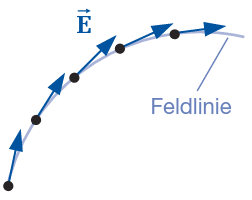
\includegraphics[scale=0.6]{../img/I/Id}}
\caption{Konstruktion der Feldlinie.}
\label{fig_Id}
\end{figure}
\noindent Die Dichte der in einem Feldlinienbild eingezeichneten Feldlinien kann in vielen Fällen sogewählt werden, dass sie ein Mass für den Betrag der Feldstärke darstellt. 
\begin{figure}[H]
\centering
\frame{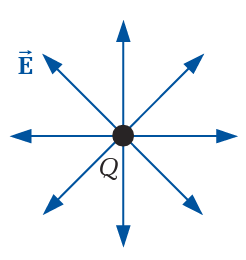
\includegraphics[scale=0.6]{../img/I/Ij}}
\caption{Feldlinienbild einerpositiven Punktladung.}
\label{fig_Ij}
\end{figure}
\noindent Die Feldlinien gehen immer von der positiven Ladungen aus und enden auf den negativen. Man nimmt an, dass die zugehörigen negativen Ladungen auf einer unendlich fernen Hülle sich befinden, ihr Beitrag zur Feldstärke wird dann bei der Berechnung vernachlässigt. Zur Vereinfachung nimmt man an,dasssich die zugehörigen negativen Ladungen auf der \textbf{unendlich fernen Hülle} befinden, ihr Beitrag zur Feldstärke wird dann bei der Berechnung vernachlässigt. Die elektrische Feldstärke zeigt radial und nach ausse und ist abhängig nur vom Abstand zur Punktladung $Q$.
\newline\newline
Einen weiteren Sondernfall bildet das \textbf{homogene Feld}, bei dem die Feldstärke überall die gleiche Richtung und den gleichen Betrag aufweist. Ein derartiges Feld lässt sich nur näherungsweise und auch nur in einem begrenzten räumlichen Bereich realisieren.
%%%%%%%%%%%%%%%%%%%%%%%%%%%%%%%%%%%%%%%%%%%%%%%%%%%%%%%%%%%%%%%%%%%%%%%%%%%%%%%%%%%%%%%%%%%%%%%%
\section{Feldbild für zwei Punktladungen}
Das Feldlinienbild zweier Punktladungen $Q_1$ und $Q_2$, die sich auf der $y$-Achse an den Stellen $y=a$ und $y=-a$ befinden wird wie folgt berechnen. Die elektrische Feldstärkein einem allgemeinen Punkte in der $xy$-Ebene wird zunächst berechnet. 
\begin{figure}[H]
\centering
\frame{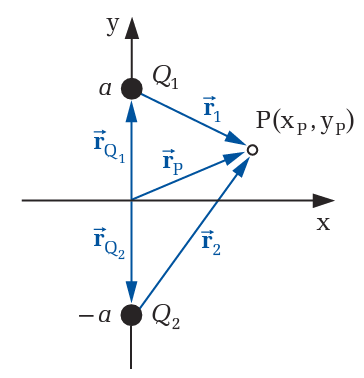
\includegraphics[scale=0.5]{../img/I/Ik}}
\caption{Feldlinienbild zweier Punkte.}
\label{fig_Ik}
\end{figure}
\begin{equation}
\boxed{
\begin{array}{lll}
\overrightarrow{r}_1&=&\overrightarrow{r}_P-\overrightarrow{r}_{Q_1}=x_P\overrightarrow{e}_x+\left(y_P-a\right)\overrightarrow{e}_y\\
\overrightarrow{r}_2&=&\overrightarrow{r}_P-\overrightarrow{r}_{Q_2}=x_P\overrightarrow{e}_x+\left(y_P+a\right)\overrightarrow{e}_y\\
r_1&=&\sqrt{x_P^2+\left(y_P-a\right)^2}\\
r_2&=&\sqrt{x_P^2+\left(y_P+a\right)^2}\\
\overrightarrow{E}\left(\overrightarrow{r}_P\right)&=&\dfrac{1}{4\pi\epsilon_0}\Bigg[Q_1\dfrac{\overrightarrow{r}_1}{r_1^3}+Q_2\dfrac{\overrightarrow{r}_2}{r_2^3}\Bigg]\\
&=&\dfrac{1}{4\pi\epsilon_0}\Bigg[\left(Q_1\dfrac{x_P}{r_1^3}+Q_2\dfrac{x_P}{r_2^3}\right)\overrightarrow{e}_x+\left(Q_1\dfrac{y_P-a}{r_1^3}+Q_2\dfrac{y_P+a}{r_2^3}\right)\overrightarrow{e}_y\Bigg]\\
\end{array}
}
\end{equation}
Die Auswertung dieser Beziehung für die beiden Sonderfälle gleicher $Q_1=Q_2=Q$ bzw. entgegengesetzt gleicher Punktladungen $Q_1=Q$, $Q_2=-Q$ ist in folgendes Bild zu betrachten.
\begin{figure}[H]
\centering
\frame{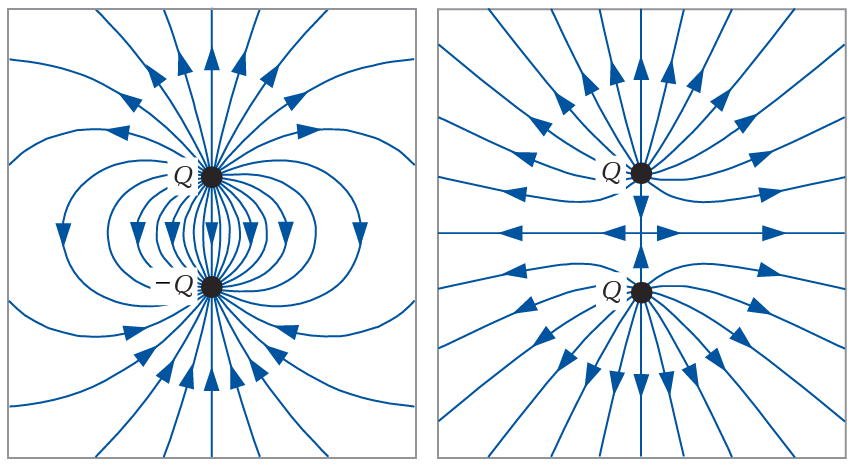
\includegraphics[scale=0.4]{../img/I/Il}}
\caption{\textbf{\textit{Links:}} sich anziehende Ladungen. \textbf{\textit{Rechts:}} sich abstossende Ladungen}
\label{fig_Il}
\end{figure}
%%%%%%%%%%%%%%%%%%%%%%%%%%%%%%%%%%%%%%%%%%%%%%%%%%%%%%%%%%%%%%%%%%%%%%%%%%%%%%%%%%%%%%%%%%%%%%%%
\section{Das elektrostatische Potential}
Eine Punktladung $Q$ kann von einem äusseren elektrischen Feld oder von anderen Ladungen eine Kraft ausüben. Soll diese Ladung von einem Punkt $P_0$ zu einem Punkt $P_1$ verschiben werden, dann muss gegen diese Feldkräfte eine Arbeit aufgewendet werden. Die erforderliche Arbeit ist
\begin{equation} 
\boxed{W_e=-\displaystyle \int_{P_0}^{P_1}\overrightarrow{F}\bullet \text{d}\overrightarrow{s}=-Q\displaystyle \int_{P_0}^{P_1}\overrightarrow{E}\bullet \text{d}\overrightarrow{s}}
\end{equation} 
\noindent Der Wert $W_e$ beschreibt die von aussen dem System zugeführte Energie. Der Sonderfall, dass eine Ladung $Q$ entlang eines geschlossenen Weges, beginnend beim Punkt $P_0$ entlang der Kontur $C_1$ zum Punkt $P_1$ und anschliessend entlang der Kontur $C_2$ wieder zurück zum Punkt $P_0$ bewegt wird. Die insgesamt geleistete Arbeit verschwindet, d.h. das Linienintegral der elektrischen Feldstärke entlang der Kontur $C_1$ ist entgegengesetzt gleich dem Linienintegral der elektrischen Feldstärke entlang der Kontur $C_2$. Die geschlossene Kontur $C$ setzt sich aus den beiden Konturen $C_1$ und $C_2$ zusammen.
\begin{figure}[H]
\frame{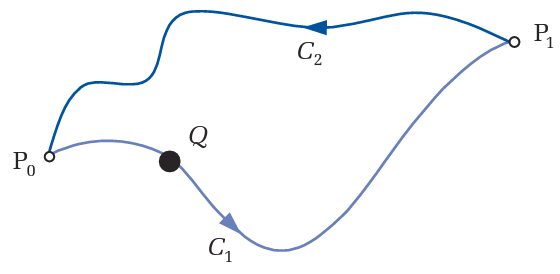
\includegraphics[scale=0.5]{../img/I/If}}
\centering
\caption{Bewegung einer Punktladung entlang eines geschlossenen Weges.}
\label{fig_If}
\end{figure}
\begin{equation}
\boxed{
\begin{array}{lll}
W_e&=&-Q\displaystyle \int_{C_1}\overrightarrow{E}\bullet \text{d}\overrightarrow{s}-Q\displaystyle \int_{C_2}\overrightarrow{E}\bullet \text{d}\overrightarrow{s}\\
&=&-Q\displaystyle \int_{P_0}^{P_1}\overrightarrow{E}\bullet \text{d}\overrightarrow{s}-Q\displaystyle \int_{P_1}^{P_2}\overrightarrow{E}\bullet \text{d}\overrightarrow{s}\\
&=&-Q\displaystyle \oint_{C}\overrightarrow{E}\bullet \text{d}\overrightarrow{s}\\
&=&0
\end{array}}
\end{equation}
Das Verschwinden des entlang einer geschlossenen Kontur gebildete Umlaufintegral im elektrostatischen Feld entsteht aus der Tatsache der Rechnung, dass die elektrischen Feldlinien bei den positiven Ladungen beginnen und bei den negativen enden. Die Ladungen stellen die Quellen für das elektrostatische Feld dar. Dieses wird daher als \textbf{Quellenfeld} bzw. \textbf{Wirbelfeld} bezeichnet.
\newline\newline
Das \textbf{Gravitationsfeld} ist auch ein Quellenfeld, wobei die Quellen in diesem Fall durch die Massen gegeben sind. Wird ein Körper der Masse $m$ gegen die Kräfte eines Gravitationsfeldes von einem Punkt $P_0$ zu einem Punkt $P_1$ bewegt, dann ist dafür eine Arbeit aufzuwenden, die zu einer Erhöhung der potentiellen Energie des Körpers um den Betrag der geleisteten Arbeit führt.
\newline\newline
Analog führt die Bewegung einer Ladung gegen die Kräfte des \textbf{elektrischen Feldes} zu einer Erhöhung der Energie dieser Ladung, die auch in diesem Fall gleich dem Betrag der geleisteten Arbeit ist. Man spricht auch hier von der \textbf{potentiellen Energie der Ladung} und beschreibt damit die Möglichkeit dieser Ladung, durch Abgabe ihrer potentiellen Energie Arbeit leisten zu können. 
\newline\newline
Der Zuwachs an potentieller Energie bei einer Bewegung der Ladung $Q$ von einem Punkt $P_0$ zu einem Punkt $P_1$ ist gegeben durch das Produkt aus dem Wert der Ladung und dem negativen Wegintegral der elektrischen Feldstärke. Das Wegintegral ist nicht von dem Verlauf des gewählten Weges, sondern vom Anfangs- und Endpunkt abhängig.
\newline\newline
Wählt man ausgehend von einem Bezugspunkt $P_0$ unterschiedliche Endpunkte für den Integrationsweg, dann unterscheiden sich die Ergebnisse bei der Berechnung der potentiellen Energie nur durch den Wert einer skalaren Grösse. Damit kann jeder Punkt des Raumes, bezogen auf diesen Bezugspunkt durch eine skalare Grösse charakterisiert werden, für die Bezeichnung $\varphi_e$ verwendet und als \textbf{elektrostatisches Potential} genannt wird mit Dimension $\text{V}$.
\begin{equation} 
\boxed{W_e=Q\cdot \left[\displaystyle \int_{P_0}^{P_1}\left(-\overrightarrow{E}\right)\bullet \text{d}\overrightarrow{s}\right]=Q\cdot \Big[\varphi_e\left(P_1\right)-\varphi_e\left(P_0\right)\Big]}
\end{equation} 
Der Zuwachs an potentieller Energie ist proportional zur Grösse der bewegten Ladung $Q$ und zur Potentialdifferenz $\varphi_e\left(P_1\right)-\varphi_e\left(P_0\right)$, die bei der Ladungsbewegung durchlaufen wird. Da in dieser Beziehung nicht das Potential selbst, sondern lediglich die Änderung des Potentials zwischen Anfangs- und Endpunkt von Bedeutung ist, kann dem gesamten Raum ein beliebiges konstantes Potential überlagert werden, ohne dass das Ergebnis davon beeinflusst wird. 
\newline\newline
Die Festlegung eines Bezugspunktes ist willkürlich und wird üblicherweise so vorgenommen, dass man der \textbf{Erde} oder auch der unendlichen fernen Hülle das Bezugspotential $\varphi_e=0$ zuordnet. Die Erdoberfläche stellt aufgrund ihrer Leitfähigkeit eine Äquipotentialfläche dar. In Schaltungen wird üblicherweise der so genannten \textbf{Masse}, d.h. dem Minusanschluss bei einer Batterie oder dem an die Schaltung angeschlossenen metallischen Gehäuse der Bezugswert $\varphi_e=0$ zugeordnet.
\newline\newline
Legt man den Anfangspunkt $P_0$ so, dass $\varphi_e\left(P_0\right)=0$ gilt, dann ist die absolute potentielle Energie einer Punktladung im Punkt $P_1$ durch die Beziehung
\begin{equation}
\boxed{W_e\left(P_1\right)=Q\Big[\varphi_e\left(P_1\right)-\underbrace{\varphi_e\left(P_0\right)}_{0}\Big]=Q\varphi_e\left(P_1\right)}
\end{equation}
Umgekehrt lässt sich das \textbf{absolute Potential} in diesem Punkt aus der Beziehung herleiten.
\begin{equation}
\boxed{\varphi_e\left(P_1\right)=\dfrac{W_e\left(P_1\right)}{Q}=-\displaystyle \int_{P_0}^{P_1}\overrightarrow{E}\bullet \text{d}\overrightarrow{s}}
\end{equation}
%%%%%%%%%%%%%%%%%%%%%%%%%%%%%%%%%%%%%%%%%%%%%%%%%%%%%%%%%%%%%%%%%%%%%%%%%%%%%%%%%%%%%%%%%%%%%%%%
\section{Das Potential einer Punktladung}
Das von einer im Ursprung des Kugelkoordinatensystems befindlichen positiven Punktladung $Q$ in einem beliebigen Punkt $P$ hervorgerufene Potential wird hier berechnet. Die radial gerichtete Feldstärke ist durch folgende Gleichung gegeben.
\begin{equation}
\boxed{\overrightarrow{F}_2=k\cdot \dfrac{Q_1Q_2}{r^2}\cdot \overrightarrow{e}_r=\overrightarrow{E}_1\cdot Q_2}\quad \boxed{\overrightarrow{E}_1=k\cdot \dfrac{Q_1}{r^2}\overrightarrow{e}_r}
\end{equation}
Bringt man eine zweite Punktladung $Q_1$ von der Stelle $r=r_1$ entgegen der Feldrichtung an die Stelle $r=r_2<r_1$, dann muss folgende Arbeit geleistet werden.
\begin{equation}
\boxed{\begin{array}{lll}
W_e&=&-Q_1\displaystyle \int_{r_1}^{r_2}\overrightarrow{E}\bullet \text{d}\overrightarrow{s}=-Q_1\displaystyle \int_{r_1}^{r_2}\underbrace{\overrightarrow{e}_r\dfrac{Q}{4\pi\epsilon_0r^2}}_{\overrightarrow{E}}\bullet \underbrace{\overrightarrow{e}_r\text{d}r}_{\text{d}\overrightarrow{s}}\\
&=&-Q_1\dfrac{Q}{4\pi\epsilon_0}\displaystyle \int_{r_1}^{r_2}\dfrac{1}{r^2}\text{d}r=-Q_1\dfrac{Q}{4\pi\epsilon_0}\left(\dfrac{-1}{r_2}+\dfrac{1}{r_1}\right)\\
&=&Q_1\left(\underbrace{\dfrac{Q}{4\pi\epsilon_0r_2}}_{\varphi_e\left(r_2\right)}-\underbrace{\dfrac{Q}{4\pi\epsilon_0r_1}}_{\varphi_e\left(r_1\right)}\right)=Q_1\varphi_e\left(r_2\right)-Q_1\varphi_e\left(r_1\right)
\end{array}}
\end{equation}
Verlegt man den Anfangspunkt $r_1$ auf die unendlich ferne Hülle $r_1\rightarrow \infty$, dann gilt mit dem dort vorliegenden Bezugspotential $\varphi_e\left(\infty\right)=0$ für die Energie der Punktladung $Q_1$ an der Stelle $r_2$
\begin{equation}
\boxed{W_e=Q_1\dfrac{Q}{4\pi\epsilon_0r_2}=Q_1\varphi_e\left(r_2\right)}\quad \boxed{\varphi_e\left(r_2\right)=\dfrac{Q}{4\pi\epsilon r_2}}
\end{equation}
\begin{figure}[H]
\frame{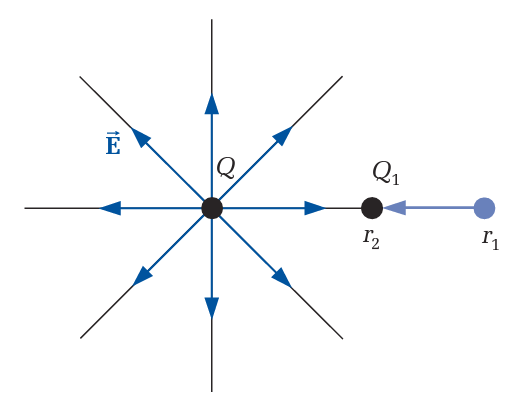
\includegraphics[scale=0.6]{../img/I/Ig}}
\centering
\caption{Verschiebung einer Punktladung im Feld einer zweiten Punktladung}
\label{fig_Ig}
\end{figure}
\noindent Der Ausdruck $\varphi\left(r_2\right)$ beschreibt das von der Punktladung $Q$ an der Stelle $r=r_2$ hervorgerufene Potential. Dieses ist proportional zur Ladung und umgekehrt proportional zum Abstand von der Ladung. Die Arbeit ist positiv, wenn beide Ladungen gleiche Vorzeichen haben und sich gegenseitig abstossen.
\\\\
Die Gleichung $W_e=Q_1\varphi_e\left(r_2\right)-Q_1\varphi_e\left(r_1\right)$ beschreibt die aufzuwendende Arbeit bzw. die Zunahme der potentiellen Energie der Punktladung $Q_1$, wenn diese von einem Punkt $r_1$ mit dem Potential $\varphi_e\left(r_1\right)$ zu einem Punkt $r_2$ mit dem Potential $\varphi_e\left(r_2\right)$  bewegt wird. Das Verschieben einer Ladung zwischen zwei Punkten mit gleichem Potential erfordert als Integral über den gesamten Weg betrachtet keine Arbeit. 
%%%%%%%%%%%%%%%%%%%%%%%%%%%%%%%%%%%%%%%%%%%%%%%%%%%%%%%%%%%%%%%%%%%%%%%%%%%%%%%%%%%%%%%%%%%%%%%%
\section{Die elektrische Spannung}
Die Potentialdifferenz zwischen zwei beliebigen Punkten $P_1$ und $P_2$ kann durch einen Bezugspunkt $P_0$ berechnet werden. Das Ergebnis ist unabhängig von der Wahl des Bezugspunktes $P_0$ und wird als elektrische Spannung $U$ zwischen den Punkten $P_1$ und $P_2$ 
\begin{equation}
\boxed{
\begin{array}{lll}
\varphi_e\left(P_1\right)-\varphi_e\left(P_2\right)&=&-\displaystyle \int_{P_0}^{P_1}\overrightarrow{E}\bullet\text{d}\overrightarrow{s}+\displaystyle \int_{P_0}^{P_2}\overrightarrow{E}\bullet\text{d}\overrightarrow{s}\\
&=&\displaystyle \int_{P_1}^{P_0}\overrightarrow{E}\bullet\text{d}\overrightarrow{s}+\displaystyle \int_{P_0}^{P_2}\overrightarrow{E}\bullet\text{d}\overrightarrow{s}\\
&=&\displaystyle \int_{P_1}^{P_2}\overrightarrow{E}\bullet\text{d}\overrightarrow{s}
\end{array}}
\end{equation}
\begin{equation}
\boxed{U_{12}=\varphi_e\left(P_1\right)-\varphi_e\left(P_2\right)=\displaystyle \int_{P_1}^{P_2}\overrightarrow{E}\bullet\text{d}\overrightarrow{s}}
\end{equation}
%%%%%%%%%%%%%%%%%%%%%%%%%%%%%%%%%%%%%%%%%%%%%%%%%%%%%%%%%%%%%%%%%%%%%%%%%%%%%%%%%%%%%%%%%%%%%%%%
\section{Die Kapazität}
Die Spannung $U$ und die Ladung $Q$ sind zueinander proportional. Diese Proportionalität gilt unabhängig von der geometrie der Anordnung. Der Proportionalitätsfaktor $C$ wird als \textbf{Kapazität} bezeichnet und hat Dimension F=As/V. 
\begin{equation}
\boxed{Q=C\cdot U}
\end{equation}
Unter der Kapazität versteht man das Verhältnis aus der aufgenommenen Ladung $Q$ zu der angelegten Spannung $U$. Sie ist ein Mass für die Fähigkeit eines Körpers, Ladungen zu speichern.
\begin{equation}
\boxed{Q=\displaystyle \oiint_{A}\overrightarrow{D}\bullet \text{d}\overrightarrow{A}=\displaystyle \oiint_{A}\sigma \,\text{d}A}\quad \boxed{U=\displaystyle \int_s\overrightarrow{E}\bullet \text{d}\overrightarrow{s}}
\end{equation}
\begin{equation}
\boxed{C=\dfrac{Q}{U}=\dfrac{\epsilon \displaystyle \oiint_{A}\overrightarrow{D}\bullet \text{d}\overrightarrow{A}}{\displaystyle \int_s \overrightarrow{E}\bullet \text{d}\overrightarrow{s}}}
\end{equation}
Während die Kapazität die Eigenschaft der Leiteranordnung (Fassungsvermögen) beschreibt, wurd eine Anordnung mit dieser Eigenschaft als \textbf{Kondensator} (als Bauelement) bezeichnet. Allgemein spricht man von einem Kondensator, wenn zwei leitende Beläge mit entgegengesetzten , gleich grossen Ladungen vorhanden sind und alle Feldlinien, d.h. der gesamte elektrische Fluss, von der mit den positiven Ladungen besetzten Fläche zu der mit den negativen Ladungen besetzten Fläche gelangen.
